



\documentclass[a4paper,12pt,spanish]{article}

\usepackage[utf8]{inputenc}


\usepackage{blindtext}
%\usepackage{microtype}
\usepackage{amsfonts, amsmath, amsthm, amssymb}
%\usepackage{fancyhdr}
%\usepackage{index}
%\usepackage{multicol}    

\usepackage[T1]{fontenc}
\usepackage[utf8]{inputenc}
\usepackage{graphicx}
\usepackage[spanish,es-tabla]{babel}
\usepackage{url}
\usepackage{enumitem}

\usepackage[unicode=true, pdfusetitle,
bookmarks=true,bookmarksnumbered=false,bookmarksopen=false,
breaklinks=true,pdfborder={0 0 1},backref=false,colorlinks=false]
{hyperref}

\usepackage{listings}


\usepackage{siunitx} %para el sistema internacional
\usepackage[export]{adjustbox}
\usepackage{booktabs} 
\usepackage{subcaption}

\usepackage{float}


\newcommand{\address}[1]{
	\par {\raggedright #1
		\vspace{1.4em}
		\noindent\par}
}


\pagenumbering{gobble}
\include{noNumberPage}
\pagenumbering{arabic}
\setcounter{page}{14}

%tutorial de tablas latex: https://manualdelatex.com/tutoriales/tablas

\usepackage{multirow}

% \usepackage[table,xcdraw]{xcolor}


%Inicio del documento (hasta que se cierre con \end{document}
\begin{document}
	
	
	\title{Conservación de la energía mecánica}
	
	%\author{Adrián Rivero Fernández}
	\date{}
	
	\maketitle
	
	
	
	\begin{abstract} %resumen
		
		
		Pretendemos estudiar la conservación de la energía mecánica de un sólido con rotación y desplazamiento, y la determinación del momento de inercia de la rueda de Maxwell.
		
		
		
	\end{abstract}
	
	\section{Introducción}
	
	La conservación de la energía mecánica viene dada por la expresión 
	\[ E= T+U\]
	que representa que la energía mecánica equivale a la suma de la cinética (T) mas la potencial (U), siendo estas 
	\[T= \frac{1}{2}mv^2 + \frac{1}{2}I\omega^2\]
	\[U = - m  g h\]
	siendo las alturas negativas y $g=(9,8\pm 0,1) \si{m/s}$
	
	Para un sólido que se desplaza verticalmente, con velocidad angular horizontal, tendremos que $\omega = \frac{v}{r}$, siendo $r$ el radio de giro. De modo que tenemos
	\[E = -mgh + \frac{1}{2}v^2(m+\frac{I}{r^2})\]
	
	Teniendo en cuenta que $v = \frac{dh}{dt}$, podemos obtener la ecuación diferencial
	\[0=-mgv + \frac{1}{2}(m+\frac{I}{r^2})v\frac{dv}{dt}\]
	
	de la que obtenemos
	\[v= \frac{mg}{m+\frac{I}{r^2}}t\]
	\[h= \frac{1}{2}\left(\frac{mg}{m+\frac{I}{r^2}}\right)t^2\]
	
	
	\section{Material y Métodos}
	
	
	%describir el aparato que hemos montado para este experimento, y el procedimiento que vamos a llevar a cabo para el medimiento, las dificultades, etc.
	
	Para realizar el experimento disponemos de una estructura formada por el pie en forma de A y una varilla horizontal, de la que cuelga la rueda de Maxwell.
	Enrollaremos la cuerda sobre la rueda y la dejaremos caer, de modo que la tensión de la cuerda produzca un torque sobre la rueda, y adquiriendo esta aceleración angular.
	
	Disponemos de un sistema para soltar la rueda que activa un contador digital, y más abajo de un sensor fotoeléctrico que detecta el eje de la rueda al caer, y para el contador.
	Hay que tener precaución de que el sensor fotovoltaico mida siempre la misma parte del eje, ya que tiene otra parte de mayor grosor, y esto podría darnos incoherencias en la toma de medidas.
	
	Mediremos el tiempo de caida para distinntas alturas, y su velocidad, y podremos estudiar la validez de las expresiones para la conservación de la energía.
	
	Hay que tener precaución, además, con que al soltar la rueda no hayan movimientos de vaivén en el disco, y que al enrollar el hilo este quede uniforme a ambos lados de la rueda, sin superposiciones, ya que de lo contrario habrá desniveles y desequilibrios que llevarán a anomalías en la toma de medidas.
	


\begin{figure}[H]
	\centering
	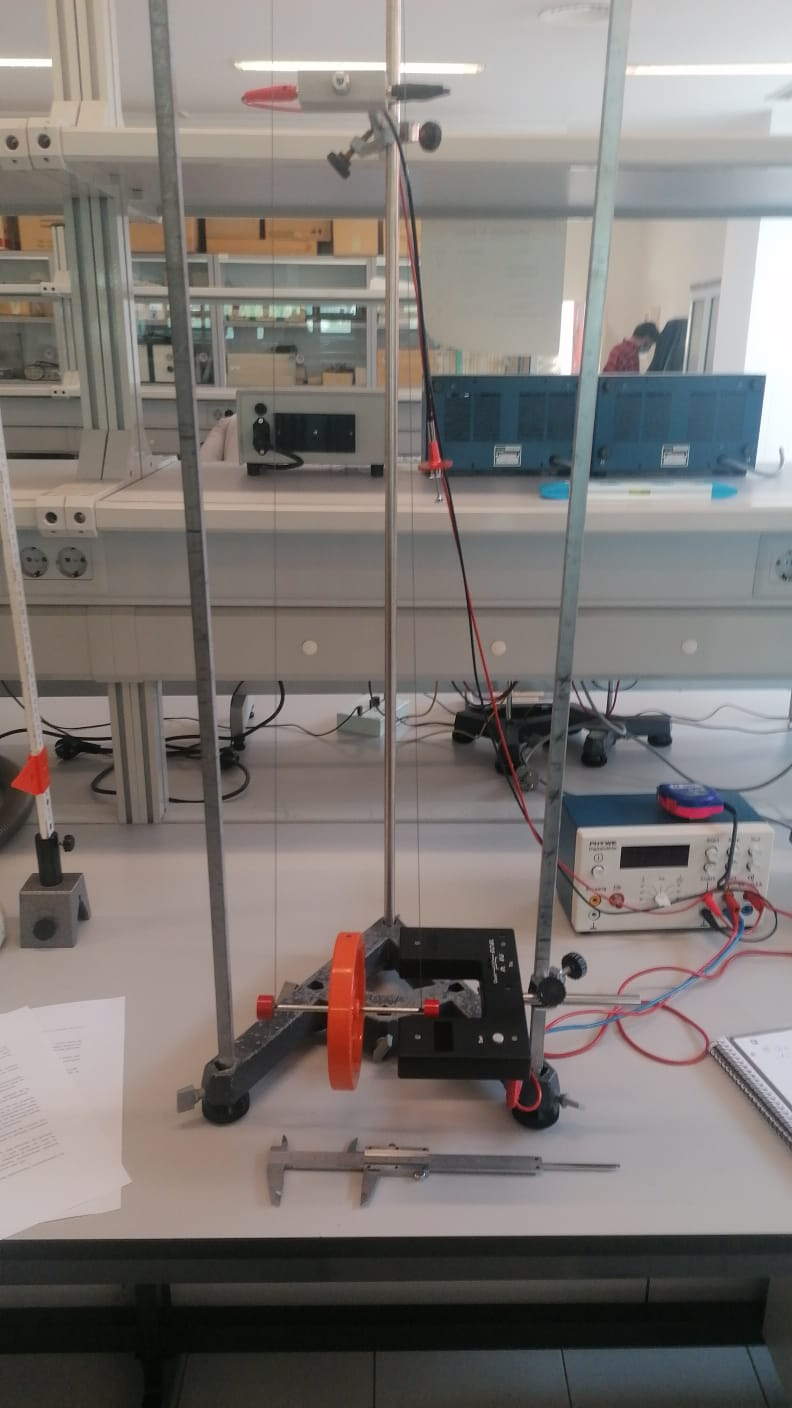
\includegraphics[width=0.8\linewidth]{../fotos/euoaoeua}
	\caption{Dispositivo experimental}
	\label{fig:euoaoeua}
\end{figure}
	
	
\begin{figure}[H]
	\centering
	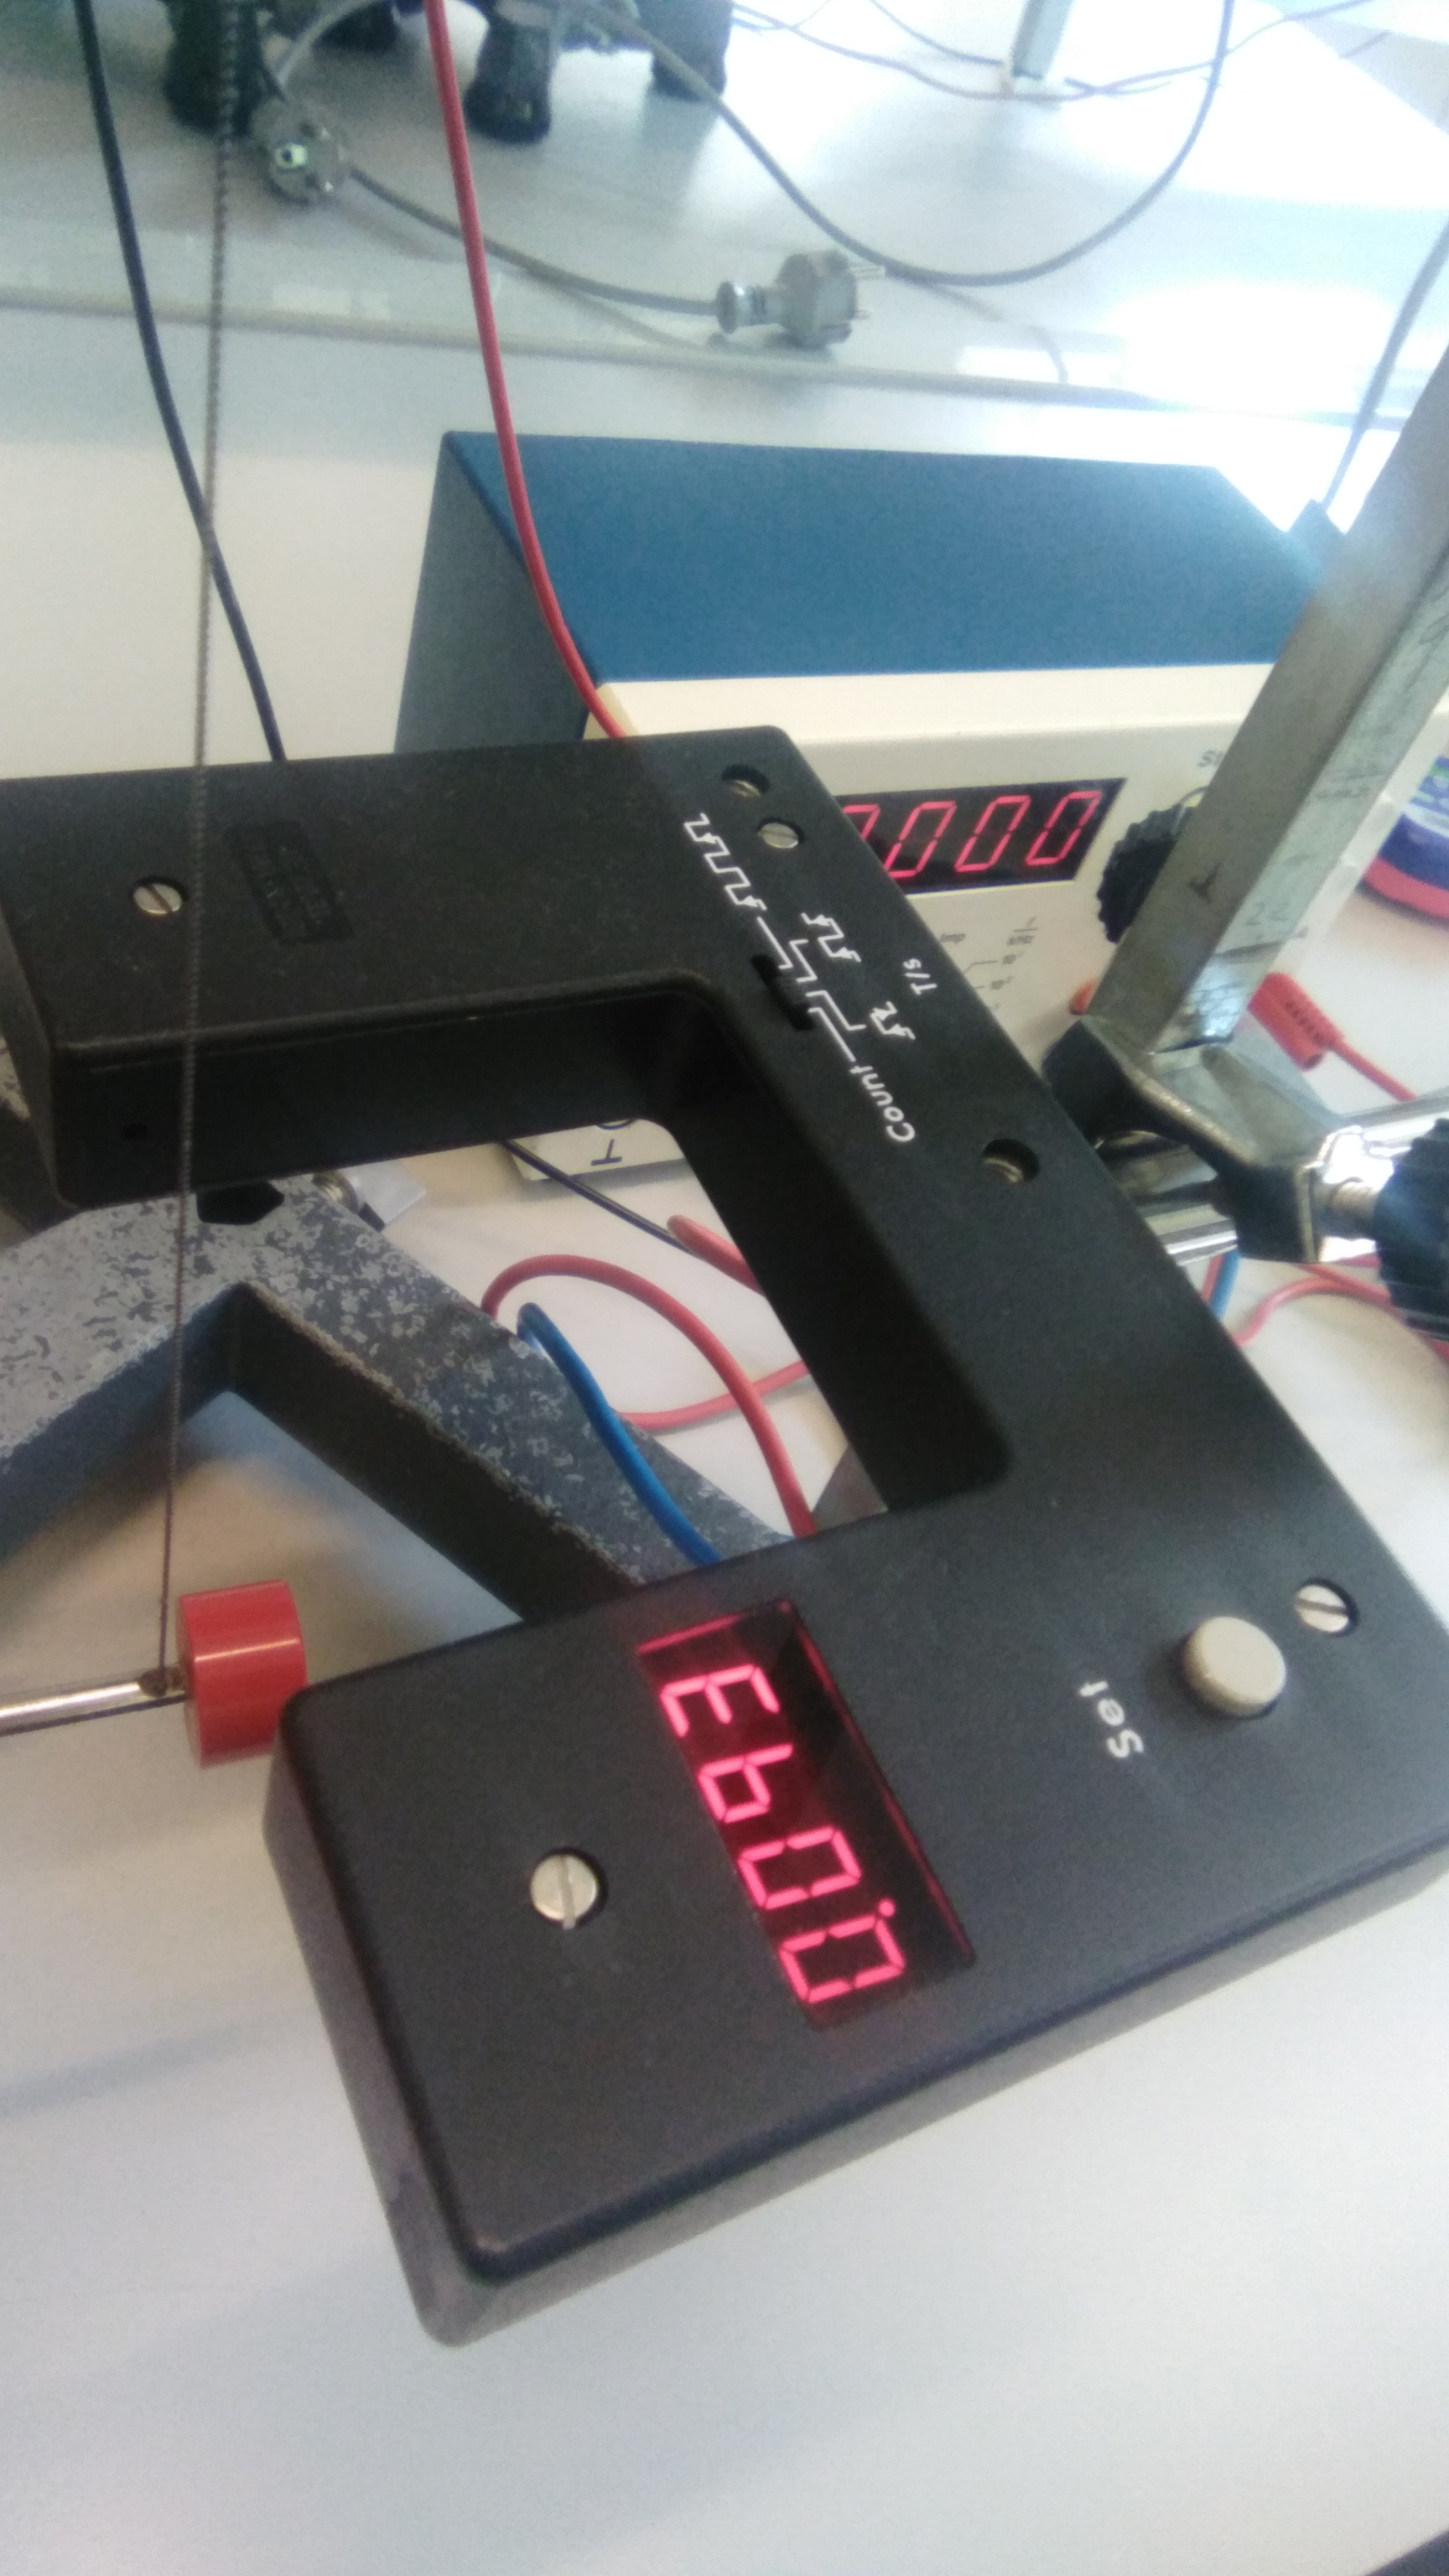
\includegraphics[width=0.8\linewidth]{../fotos/IMG_20220430_105309}
	\caption{medidor digital con el eje que debe detectar}
	\label{fig:img20220430105309}
\end{figure}


	\section{Resultados}
	
		
	\begin{itemize}
	\item{ Diámetro: 0,054$\pm$ 0,001 m }
	\item{ Radio: 0,0270$\pm$ 0,0005 m }
	\item{ Masa: 0,365$\pm$ 0,001 Kg }
	\item{ g: 9,81$\pm$ 0,01 m/s}
	\end{itemize}
	
	
Hemos tomado 10 alturas, repitiendo la toma de datos 3 veces para cada una y calculando la media.
El error en la media podemos obtenerlo mediante
\[\Delta T = \sqrt{\frac{\sum(\bar t-t_i)}{N(N-1)}}\]

	\begin{itemize}
	\item{Error en la altura: $0,001 \si{m}$}
	\item{Error en el tiempo: $0,001 \si{s}$}
\end{itemize}

Los datos obtenidos están recogidos en la Tabla 1.



\begin{table}[H]
	\begin{minipage}[t]{.48\linewidth}
		\centering
		\begin{tabular}{|l|l|}
			\hline
			\textbf{Altura (m)}         & \textbf{0,6}   \\ \hline
			Tiempo 1 (s)      & 6,563 \\ \hline
			Tiempo 2 (s)      & 6,56  \\ \hline
			Tiempo 3 (s)      & 6,547 \\ \hline
			Tiempo medio (s)  & 6,557 \\ \hline
			Error de la media & 0,005 \\ \hline\hline
			\textbf{Altura (m)}         & \textbf{0,55}   \\ \hline
			Tiempo 1 (s)      & 6,275 \\ \hline
			Tiempo 2 (s)      & 6,184 \\ \hline
			Tiempo 3 (s)      & 6,275 \\ \hline
			Tiempo medio (s)  & 6,24  \\ \hline
			Error de la media & 0,03  \\ \hline\hline
			\textbf{Altura (m)}         & \textbf{0,5}   \\ \hline
			Tiempo 1 (s)      & 5,986 \\ \hline
			Tiempo 2 (s)      & 5,923 \\ \hline
			Tiempo 3 (s)      & 5,946 \\ \hline
			Tiempo medio (s)  & 5,95  \\ \hline
			Error de la media & 0,02  \\ \hline\hline
			\textbf{Altura (m)}         & \textbf{0,45}   \\ \hline
			Tiempo 1 (s)      & 5,663 \\ \hline
			Tiempo 2 (s)      & 5,674 \\ \hline
			Tiempo 3 (s)      & 5,668 \\ \hline
			Tiempo medio (s)  & 5,668 \\ \hline
			Error de la media & 0,003 \\ \hline\hline
			\textbf{Altura (m)}         & \textbf{0,4}   \\ \hline
			Tiempo 1 (s)      & 5,363 \\ \hline
			Tiempo 2 (s)      & 5,358 \\ \hline
			Tiempo 3 (s)      & 5,265 \\ \hline
			Tiempo medio (s)  & 5,33  \\ \hline
			Error de la media & 0,03  \\ \hline
		\end{tabular}
		
	\end{minipage}\hfill
	\mbox{}
	\begin{minipage}[t]{.48\linewidth}% -----------------------tabla 2
		\centering
		\begin{tabular}{|l|l|}
			\hline
			\textbf{Altura (m)}         & \textbf{0,35}   \\ \hline
			Tiempo 1 (s)      & 5,039 \\ \hline
			Tiempo 2 (s)      & 5,017 \\ \hline
			Tiempo 3 (s)      & 5,021 \\ \hline
			Tiempo medio (s)  & 5,026 \\ \hline
			Error de la media & 0,007 \\ \hline\hline
			\textbf{Altura (m)}         & \textbf{0,3}   \\ \hline
			Tiempo 1 (s)      & 4,664 \\ \hline
			Tiempo 2 (s)      & 4,592 \\ \hline
			Tiempo 3 (s)      & 4,677 \\ \hline
			Tiempo medio (s)  & 4,64  \\ \hline
			Error de la media & 0,03  \\ \hline\hline
			\textbf{Altura (m)}         & \textbf{0,25}   \\ \hline
			Tiempo 1 (s)      & 4,213 \\ \hline
			Tiempo 2 (s)      & 4,24  \\ \hline
			Tiempo 3 (s)      & 4,233 \\ \hline
			Tiempo medio (s)  & 4,229 \\ \hline
			Error de la media & 0,008 \\ \hline\hline
			\textbf{Altura (m)}         & \textbf{0,2}   \\ \hline
			Tiempo 1 (s)      & 3,773 \\ \hline
			Tiempo 2 (s)      & 3,879 \\ \hline
			Tiempo 3 (s)      & 3,873 \\ \hline
			Tiempo medio (s)  & 3,84  \\ \hline
			Error de la media & 0,03  \\ \hline\hline
			\textbf{Altura (m)}         & \textbf{0,15}   \\ \hline
			Tiempo 1 (s)      & 3,343 \\ \hline
			Tiempo 2 (s)      & 3,205 \\ \hline
			Tiempo 3 (s)      & 3,258 \\ \hline
			Tiempo medio (s)  & 3,27  \\ \hline
			Error de la media & 0,04  \\ \hline
		\end{tabular}
		
	\end{minipage}\hfill
	\mbox{}
	\caption{Semiperiodo de las masas según distancias}
\end{table}


	
	\section{Discusión}
	
	Aplicando la expresión
	\[E = -mgh + \frac{1}{2}v^2(m+\frac{I}{r^2})\]
	
	entre el punto más alto y el más bajo, podemos despejar la inercia de modo que 
	\[  -mgh = \frac{1}{2}v^2(m+\frac{I}{r^2})
	\]
	Teniendo en cuenta que 
	\[v= \frac{mg}{m+\frac{I}{r^2}}t\]
	
	tenemos que 
	\[ I = \frac{r^2(\frac{1}{2} m^2g^2t^2 + m^2gh)}{mgh}\]
	
	Los resultados quedan recogidos en la Tabla 2.
	Vemos que el resultado de la inercia media nos da
	\[ \boxed{I_{1} = (0,000936 \pm 0,000004) \si{kg \cdot m^2}}\]
	
	\begin{table}[H]
		\centering
		\begin{tabular}{|c|c|}
			\hline
			\textbf{Altura (m)} & \textbf{Inercia ($\si{kg \cdot m^2}$)} \\ \hline
			0,6                 & 0,000932         \\ \hline
			0,55                & 0,000923         \\ \hline
			0,5                 & 0,000922         \\ \hline
			0,45                & 0,000929         \\ \hline
			0,4                 & 0,000929         \\ \hline
			0,35                & 0,000945         \\ \hline
			0,3                 & 0,000941         \\ \hline
			0,25                & 0,000936         \\ \hline
			0,2                 & 0,000966         \\ \hline
			0,15                & 0,000932         \\ \hline\hline
		\textbf{	Media }              & 0,000936         \\ \hline
			\textbf{Error en la media}   & 0,000004         \\ \hline
		\end{tabular}
	\caption{Inercia}
	\end{table}
	
	La Figura 3 representa $h$ frente a $t^2$. La recta de ajuste es
	\[ y = Ax + B  \]
	\[A = 0,0142 \pm 0,00010(\si{m/s^2}) \]
	\[B = -0,004 \pm 0,003 (\si{m})\] 


\begin{figure}[H]
	\centering
	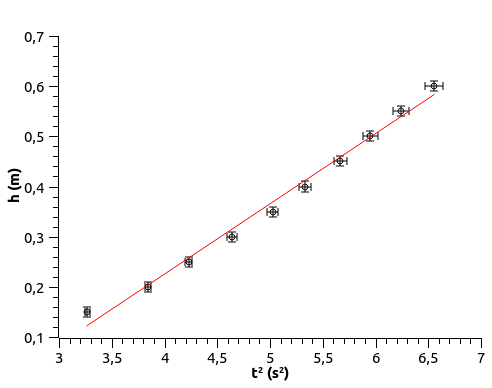
\includegraphics[width=1\linewidth]{grafica3}
	\caption{$h$ frente a $t^2$}
	\label{fig:grafica1}
\end{figure}

siguiendo la expresión de $h$ en función de $t^2$, podemos entender que la pendiente $A$ del ajuste, ya que $h = At^2$ es 
\[A = \frac{1}{2}\left(\frac{mg}{m+\frac{I}{r^2}}\right)\]
Por lo que la inercia la despejamos como
\[ I = \left( \frac{ m g}{2A}- m \right)r^2 \]

y propagando el error:
\[\Delta I =  \left( \frac{- m g r^2}{2A^2} \right) \Delta A \]
siendo 

% +  \left( \frac{A g r^2}{2} -1 \right) \Delta m + \left( \frac{A m r^2}{2}  \right) \Delta g + \left( \frac{2 A m g r}{2}  \right) \Delta r 

%I = 0,0009164567

\[\boxed{ I_2 = 0,000916 \pm 0,000006 \si{kg \cdot m^2}} \]

Ahora, representamos en la Figura 4 $v$, calculada mediante $v= \frac{h}{t}$, frente a $t$

\begin{figure}[H]
	\centering
	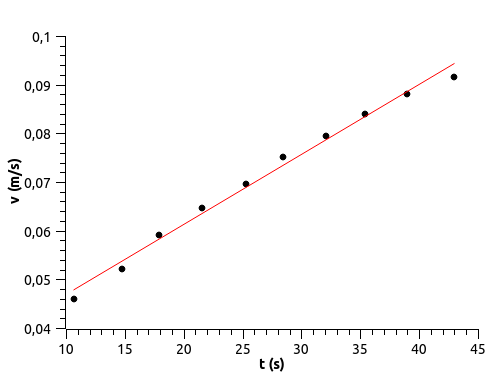
\includegraphics[width=1\linewidth]{grafica2}
	\caption{$v$ frente a $t$}
	\label{fig:grafica2}
\end{figure}

Igual que antes, ajustamos por mínimos cuadrados y obtenemos 

\[ y = Ax+B\]
\[A = 0,0143  \pm  0,0002 (\si{m/s^2}) \]
\[B = -0,002 \pm  0,0011  (\si{m/s}) \]

Esta vez tenemos que 
\[A = \frac{mg}{m+\frac{I}{r^2}} \]
de modo que 
\[I = \left(\frac{mg}{A}- m\right) r^2\]
\[\Delta I = \left|\frac{ - mg r^2}{A^2} \right| \Delta A \]

%\[ I_3 = 0,00182 \pm 0,00003    \]
\[ \boxed{I_3 = 0,00182 \pm 0,00003  \si{kg \cdot m^2}  }\]



	\section{Cuestiones}
	
	\textbf{¿Existe una gran diferencia entre los momentos de inercia calculados de diferente manera? Si hay diferencias, comente su significado y
		adjunte una posible causa.}
	
	Los valores de las dos primeras inercias son suficientemente similares, aunque se salen de sus respectivos márgenes de error, esto debe ser debido a las diferencias en los métodos empleados para su cálculo.
	En cuanto al tercero, es aproximadamente el doble que los anteriores, y si observamos las expresiones, tiene sentido que sea debido a usarse la expresión $v= h/t$.
	
	\vspace{\baselineskip}
	
	\textbf{Estime los errores asociados a los valores de I calculados con el ajuste por mínimos cuadrados.}

	Estos errores ya han sido calculados en el apartado anterior:
	\[ \Delta I_1 = (0,000004) \si{kg\cdot m^2}
	\] % UNIDADES
	\[ \Delta I_2 = (0,000006) \si{kg\cdot m^2}
	\]
	\[ \Delta I_3 = (0,00003) \si{kg\cdot m^2}
	\]
	
	\vspace{\baselineskip}
	
	\textbf{A la hora de representar gráficas se han pedido varias de ellas frente
		a valores al cuadrado, ¿por qué se piden estas gráficas en esta extraña
		representación y no frente a sus valores sin elevar al cuadrado?}
	
	Esto es debido a que en las expresiones utilizadas para despejar I, estas magnitudes vienen en estas potencias concretas, y por tanto la relación lineal se da de esta forma.
	
	\vspace{\baselineskip}
	
	\textbf{¿Por qué se consideran alturas negativas en la ecuación (3.3) de la
		energía potencial?}
	
	Es un tanto arbitrario, podríamos haber puesto un signo más a la expresión de U y tomar alturas positivas. En este caso, tomamos alturas negativas considerando la coordenada 0 la posición superior, la que inicia la cuenta del tiempo cuando cae la masa.
	

	
	
	%%%%%%%%%%%%%%%%%%%%%%%%%%%
	\begin{thebibliography}{3}
		%%%%%%%%%%%%%%%%%%%%%%%%%%%
		
		
		\bibitem{UNED2022} (varios) Guiones de prácticas- Técnicas Experimentales II. Grado en Física. Versión 2.1  UNED, 2022 \url{https://2022.cursosvirtuales.uned.es/o/3754218}
		
		
		\bibitem{UNED2021} (varios) Técnicas Experimentales I. Versión 3.5.  UNED, 2021 \url{https://2021.cursosvirtuales.uned.es/o/42035617}
		
		
		%\bibitem{2021} NOAA National Centers for Environmental Information (NCEI) \url{ https://www.ngdc.noaa.gov/ }
		
		
		
	\end{thebibliography}
	
	
	
	
	
	
\end{document}